\documentclass{article}
\usepackage{amsmath,amssymb,graphicx}
\begin{document}
\title{Computing the Delay Response from Reflectometry}
\author{Aaron Ewall-Wice}
\date{January 13th 2015}
\maketitle
Here is a brief description of how I compute the delay response of the HERA dish from reflectometry measurements. 

According to Nipanjana's memo, the reflection coefficient measured by the VNA is given by 
\begin{equation}
S_{11}(f)=\Gamma_f(f) + \frac{(1-\Gamma_f(f))^2}{\Gamma_f(f)} \sum_{n=1} \left[ \Gamma_f(f) \Gamma_d(f) e^{2 \pi i f \tau} \right]^n
\end{equation}
where $\Gamma_f(f)$ is the frequency dependent reflection coefficient of the feed and $\Gamma_d(f)$ is the reflection coefficient of the dish, and $\tau$ is the round trip delay between the feed and the dish. Because the terms in the sum are all multiplied by at least a factor of $e^{2 \pi i \tau}$ which translates them to $\tau \approx 30$\,ns in delay space, only the $\Gamma_f(f)$ out front adds significant power to the zero delay modes. 

Meanwhile, the voltage gain of the antenna, which we are trying to measure is given by 
\begin{equation}
G(f) = (1-\Gamma_f(f)) + (1-\Gamma_f(f)) \sum_{n=1} \left[\Gamma_f(f) \Gamma_d(f) e^{2 \pi i f \tau} \right]^n
\end{equation}
In the reflectometry measurement of the feed only, we measure $\Gamma_f(f)$ directly, e.g.
\begin{equation}
S_{11}^f = \Gamma_f(f)
\end{equation}
We can than obtain $\widehat{G}(f)$ through the following transformation in the frequency domain
\begin{equation}\label{eq:estimate:YesZ}
\widehat{G}(f) = \frac{\Gamma_f(f)}{1-\Gamma_f(f)} \left[S_{11}(f) - \Gamma_f(f) \right] + \left[1-\Gamma_f(f) \right]
\end{equation},
where $\Gamma_f$ is supplied directly by the feed only reflectometry measurement, $S_{11}^f$. 
Since the 
At zero delay, the amplitude of $\widetilde{G}(\tau)$ should be $\sim (1-\widetilde{\Gamma}_f(\tau))$ which we have accounted for in our calculation. In delay space, we should therefor normalize all $\tau>0$ measurements to this value. 

One can also ignore the zero delay contribution and obtain a very similar estimate where $(1-\Gamma_f(f))$ has not been added back in. We refer to this as "nz", short for "no zero". 

\begin{equation}\label{eq:estimateNoZ}
\widehat{G}_{nz}(f) = \frac{\Gamma_f(f)}{(1-\Gamma_f(f))} \left[ S_{11}(f) - \Gamma_f(f) \right]
\end{equation}


This is a fine approximation for $\tau\gtrsim 30\,$ns if one is simply looking at the delay spectrum of the voltage response but, as we will explain below, neglecting the zero delay will bias the power kernel by multiplying by an incorrect normalization factor as we will explain below. First, let's see what the data looks like.

In Fig.~\ref{fig:Reflectometry}, we plot the We note that both the feed only measurement and the feed and dish measurement level off at a similar level above  $125$\,ns, indicating that either the large time scale shallow falloff in the measurements is an intrinsic property of the feed (and not associated with feed-dish reflections) or is associated with some measurement systematic (such as reflections within the cable. We also see that the zero delay peak in the $S_{11}$ measurement of the feed and dish corresponds with the peak of the $S_{11}$ measurement of the feed only due to the fact that the first peak in both measurements arises from the reflection of the reflectometry pulse off the back of the back of the feed. 

Because the measurement of the feed only has large delay structure that is comparable to the structure in the measurement of the feed and dish, added $(1-\Gamma_f(f))$ does cause $\widehat{G}$ to be several dB larger than $\widehat{G}_{nz}$ at a few of places at large delay but the differences are not terribly dramatic. 


\begin{figure}
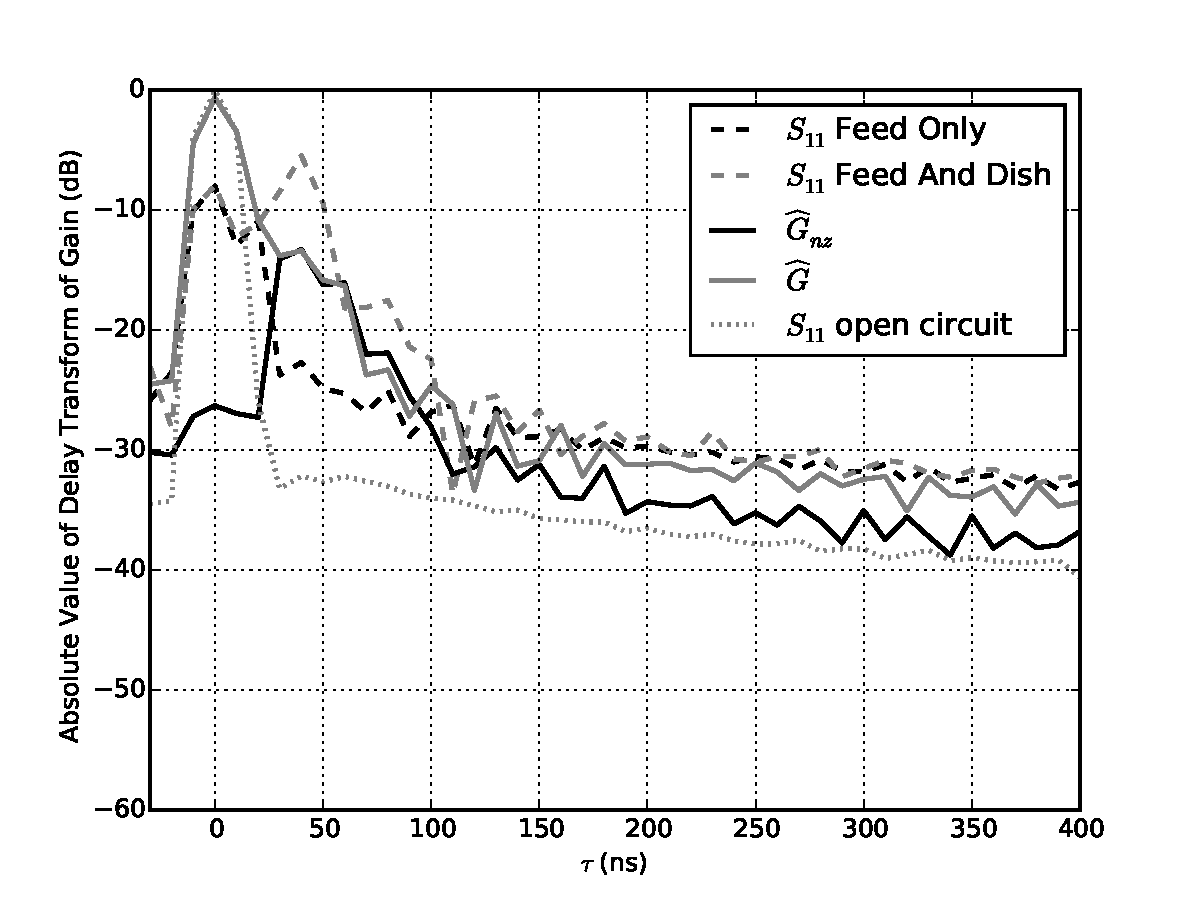
\includegraphics[width=\textwidth]{figures/GB_reflectometry.pdf}
\caption{A comparison between the one dimensional delay transform of various reflectometry measurements. The raw measurements are given by $S_{11}$ of the feed only (black dashed line) and $S_{11}$ of the feed and dish (grey dashed line). We also plot $\widehat{G}$  (solid grey line) and $\widehat{G}_{nz}$ (solid black line).  }
\label{fig:Reflectometry}
\end{figure}
 
 
 The significant disagreement between $\widehat{G}$ and $\widehat{G}_{nz}$ at zero delay, which might seem inconsequential, becomes important when one attempts to measure the power kernel. The power kernel is given by
 \begin{equation}
 \widehat{K}(\tau) = \int d \Delta \tau \widehat{G}(\Delta \tau) \widehat{G}^*(-\tau + \Delta \tau) 
 \end{equation}
Because $G(\tau)$ is a function that decreases rapidly from its maximum value at $\tau=0$, this convolution can be approximated to first order as
\begin{equation}
\widehat{K}(\tau) \approx \widehat{G}(0) \widehat{G}^*(-\tau)
\end{equation}
Hence, our estimate of $\widehat{G}(0)$ sets the overall amplitude of our estimate of $\widehat{K}(\tau)$. Because $\widehat{G}_{nz}$ does not attempt to make an accurate estimate of the zero delay mode and has subtracted it from the data, this suppresses the amplitude of $\widehat{K}_{nz}(\tau)$ by a factor of $-15$\,dB, the amplitude of $\widehat{G}_{nz}(0)$. 



\begin{figure}
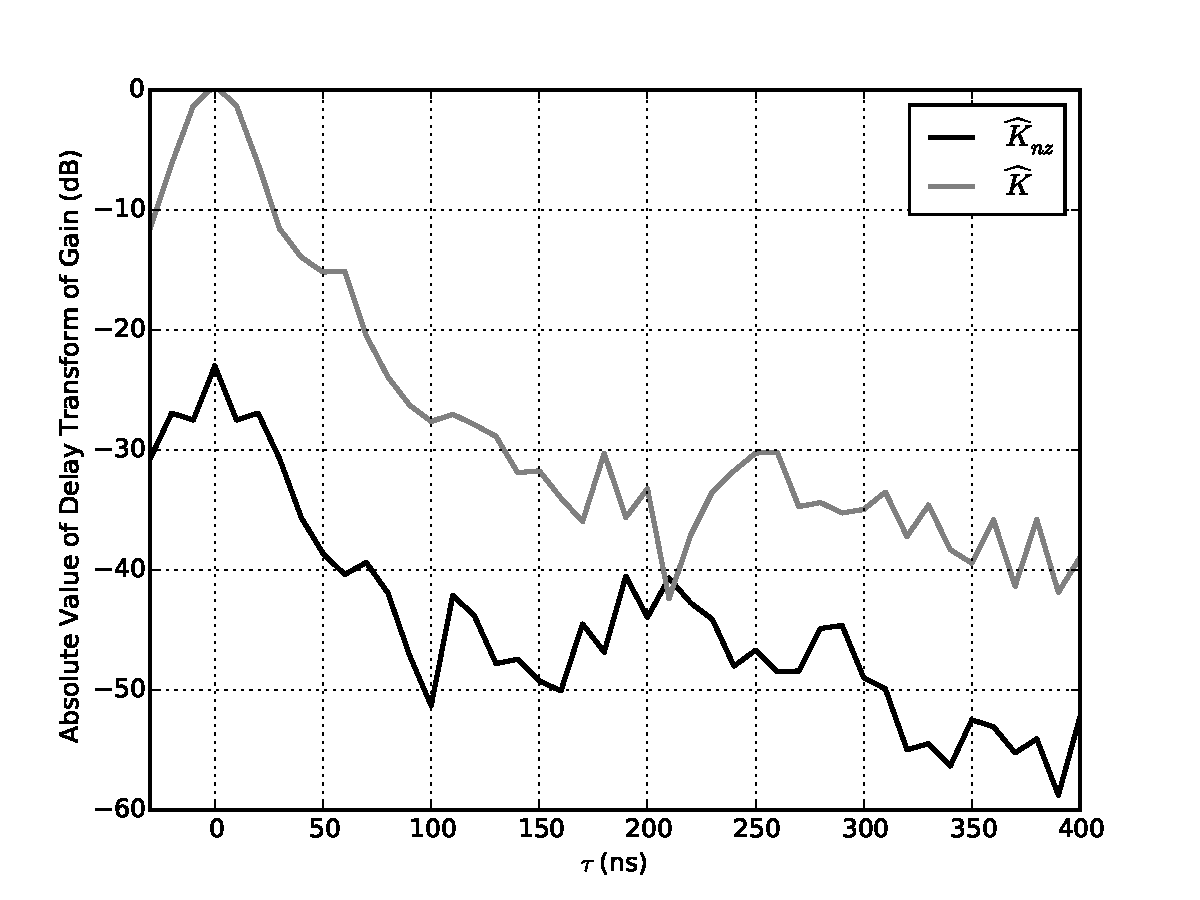
\includegraphics[width=\textwidth]{figures/GB_kernels.pdf}
\caption{A comparison between the power kernels computed with and without the inclusion of power at zero delay before performing the convolution. While the 1-dimensional voltage responses are at similar levels in Fig.~\ref{fig:Reflectometry}, they differ dramatically (by 15\,dB) in the power kernel. This is due to the difference in normalization in the convolution caused by misestimating the zero delay power.}
\label{fig:Reflectometry}
\end{figure}


\end{document}